% 7 ---------------------------------------------------------------------------
\begin{frame}{Lloyd's Algorithm}
  \begin{enumerate}\spaceditems
    \item Choose $K$ initial centers $\mu_1,\ldots,\mu_K$.
    \item \textbf{Assignment:} $z_i\leftarrow\argmin_k\norm{x_i-\mu_k}^2$.
    \item \textbf{Update:} $\mu_k\leftarrow\frac{1}{|C_k|}\sum_{i:z_i=k}x_i$.
    \item Repeat until assignments, centers, or $J$ stop changing.
  \end{enumerate}
\end{frame}

% 8 ---------------------------------------------------------------------------
\begin{frame}{A 2-D K-means Demo in the Browser}
  \centering
  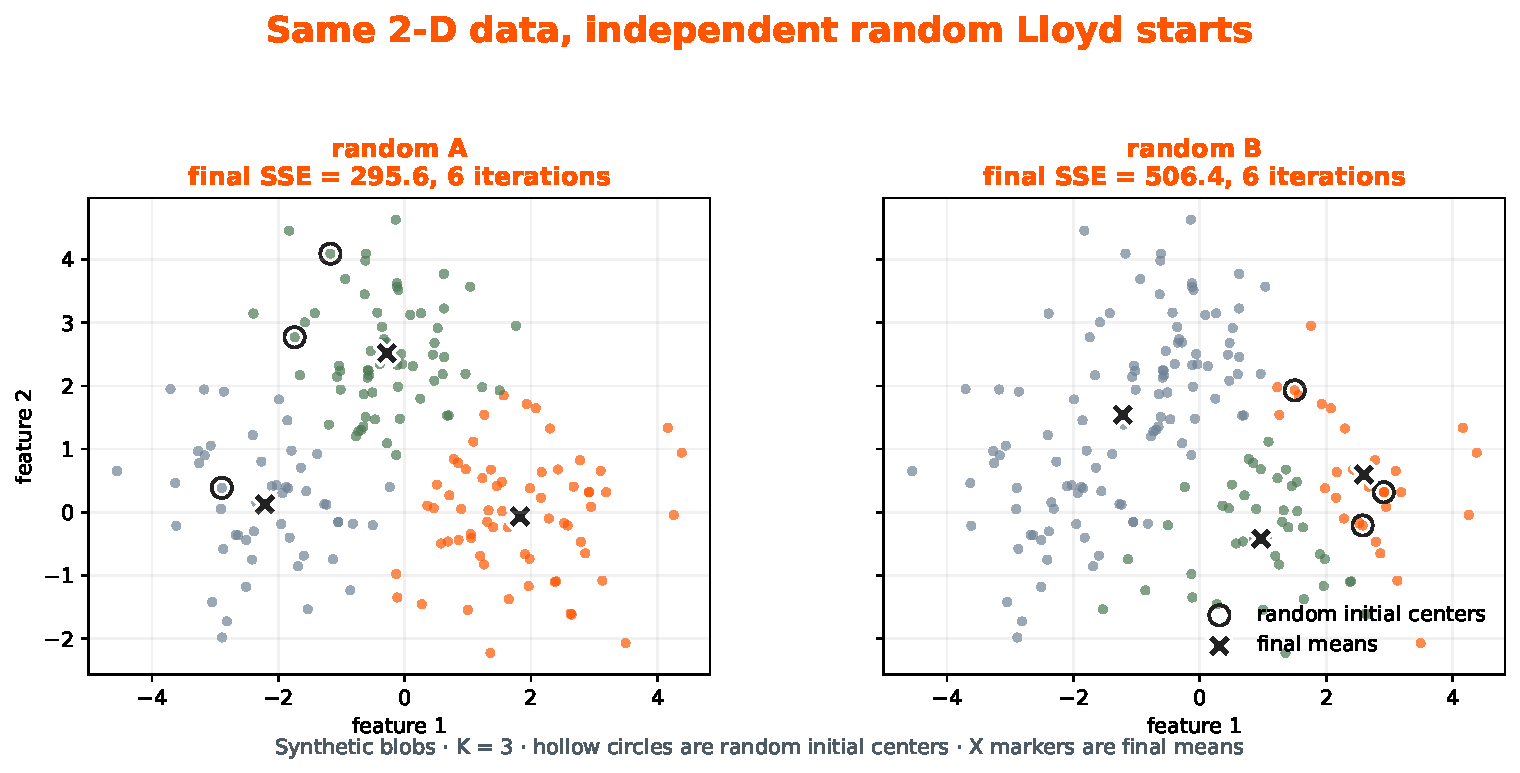
\includegraphics[width=.80\textwidth]{assets/fig_initialization_demo.pdf}
  \vspace{.01cm}
\end{frame}

% 9 ---------------------------------------------------------------------------
\begin{frame}{The Assignment Step Creates Voronoi Cells}
  \begin{columns}[c,onlytextwidth]
    \column{.52\textwidth}
      \begin{tikzpicture}[x=.50cm,y=.50cm]
        \fill[softgreen] (0,0) -- (5.8,0) -- (5.8,6) -- (0,6) -- cycle;
        \fill[softorange] (5.8,0) -- (11.5,0) -- (11.5,6) -- (5.8,6) -- cycle;
        \draw[->] (0,0)--(12,0) node[right]{$x_1$};
        \draw[->] (0,0)--(0,6.4) node[above]{$x_2$};
        \draw[dashed,thick] (5.8,0)--(5.8,6);
        \node[center] at (3,2.1) {};
        \node[center] at (8.8,3.7) {};
        \node at (3,.7) {$\mu_a$};\node at (8.8,.7) {$\mu_b$};
        \foreach \x/\y in {1/1.4,2/2.8,3.5/1.8,4.4/4.5,7/2.3,8/4.8,9.5/3.1,10.5/5.2}{\fill[black] (\x,\y) circle (2pt);}
      \end{tikzpicture}
    \column{.42\textwidth}
      A point belongs to the center with the smaller squared distance.
      \[
        \norm{x-\mu_a}^2\le \norm{x-\mu_b}^2.
      \]
      \pause
      The boundary is a hyperplane; K-means \textcolor{red}{cannot} express arbitrary non-convex cells.
  \end{columns}
\end{frame}

% 10 --------------------------------------------------------------------------
\begin{frame}{Why Does Lloyd's Objective Decrease?}
  \begin{columns}[T,onlytextwidth]
    \column{.47\textwidth}
      \textbf{Assignment step}
      \[
        J(z^{t+1},\mu^t)\le J(z^t,\mu^t).
      \]
      Each sample chooses its nearest current center.
    \column{.47\textwidth}
      \textbf{Update step}
      \[
        J(z^{t+1},\mu^{t+1})\le J(z^{t+1},\mu^t).
      \]
      Each center becomes the best mean for its current cluster.
  \end{columns}
  \pause
  \vspace{.35cm}
  \[
    J^0\ge J^1\ge J^2\ge\cdots\ge0.
  \]
  \centering
  Monotone descent gives a fixed point, not a guarantee of the global optimum.
\end{frame}
